\documentclass[twoside]{report2}
\usepackage[a4paper,width=15cm,top=2cm,bottom=2cm,bindingoffset=14mm]{geometry}

\usepackage[utf8]{vietnam}
\usepackage{lipsum}
%\usepackage{showframe}
\setlength{\parindent}{0pt}

\usepackage[framemethod=TikZ]{mdframed}

\usepackage{color}
\usepackage{listings}


\usepackage{scrextend}
\changefontsizes[17pt]{13pt}




\usepackage{mathptmx}	% same Time New Roma
%\usepackage{microtype}
%\usepackage{fontspec}
%\setmainfont{TimesNewRoman}
%\setsansfont{Arial}



\usepackage{bkthesis}
\crname{BÁO CÁO BÀI TẬP LỚN}
\ctname{HỌC PHẦN: KỸ THUẬT LẬP TRÌNH}




\definecolor{dkgreen}{rgb}{0,0.6,0}
\definecolor{gray}{rgb}{0.5,0.5,0.5}
\definecolor{mauve}{rgb}{0.58,0,0.82}
\definecolor{mycolor1}{rgb}{0.86, 0.86, 0.86}

\lstset{frame=tb,
  language=C,
  aboveskip=3mm,
  belowskip=3mm,
  showstringspaces=false,
  columns=flexible,
  basicstyle={\small\ttfamily},
  numbers=none,
  numberstyle=\tiny\color{gray},
  keywordstyle=\color{blue},
  commentstyle=\color{dkgreen},
  stringstyle=\color{mauve},
  breaklines=true,
  breakatwhitespace=true,
  tabsize=3,
  numbers=left,
  backgroundcolor=\color{mycolor1},
  rulecolor=\color{blue}, 
  stepnumber=1, 
}
%--------------------------------------
\newcounter{dinhly}[section] \setcounter{dinhly}{0}
\renewcommand{\thedinhly}{}
\newenvironment{dinhly}[2][]{%
\refstepcounter{dinhly}%
\ifstrempty{#1}%
{\mdfsetup{%
frametitle={%
\tikz[baseline=(current bounding box.east),outer sep=0pt]
\node[anchor=east,rectangle,fill=blue!50]
{\strut Định lý~\thedinhly};}}
}%
{\mdfsetup{%
frametitle={%
\tikz[baseline=(current bounding box.east),outer sep=0pt]
\node[anchor=east,rectangle,fill=blue!40]
{\strut Bài 3 - Thiết kế và viết chương trình};}}%
}%
\mdfsetup{innertopmargin=10pt,linecolor=blue!50,%
linewidth=2pt,topline=true,%
frametitleaboveskip=\dimexpr-\ht\strutbox\relax
}
\begin{mdframed}[]\relax%
\label{#2}}{\end{mdframed}}
%--------------------------------------
%\usetikzlibrary{shapes.geometric, arrows}
\usepackage{tikz}



\usepackage{amsmath}
\usepackage{amssymb}
\usepackage[colorlinks=true,breaklinks]{hyperref}

\usepackage{xcolor}
\definecolor{c1}{rgb}{0,0,1} % blue
\definecolor{c2}{rgb}{0,0.3,0.9} % light blue
\definecolor{c3}{rgb}{0.3,0,0.9} % red blue
\hypersetup{
    linkcolor={c1}, % internal links
    citecolor={c2}, % citations
    urlcolor={c3} % external links/urls
}
\usepackage{graphicx}



%--------------------------------------
\usepackage{fancyhdr}
\fancyhf{}
\renewcommand{\chaptermark}[1]{\markboth{#1}{}}
\renewcommand{\sectionmark}[1]{\markright{\thesection\ #1}}
\fancyhead[LE,RO]{{\normalsize \thepage}}
\fancyhead[LO]{{\emph{\normalsize Nhóm 10}}}
\fancyhead[RE]{\emph{{\normalsize Kỹ thuật lập trình}}}
\fancyfoot[CE,CO]{{\normalsize \thepage}}
\renewcommand{\headrulewidth}{0.4pt}
%\renewcommand{\footrulewidth}{0.4pt}
\addtolength{\headheight}{0.5pt}

\usepackage{tocloft,calc}
\renewcommand{\cftchappresnum}{Chương }
\AtBeginDocument{\addtolength\cftchapnumwidth{\widthof{\bfseries Chương }}}





\tikzstyle{startstop} = [rectangle, rounded corners, text width=3cm, minimum height=1cm,text centered, draw=red, fill=red!60]
\tikzstyle{io} = [trapezium, trapezium left angle=70, trapezium right angle=110, minimum width=3cm, minimum height=1cm, text centered, draw=black, fill=blue!30]
\tikzstyle{process} = [rectangle, text width=3cm, minimum height=1cm, text centered, draw=orange, fill=orange!60]
\tikzstyle{decision} = [diamond, minimum width=3cm, minimum height=1cm, text centered, draw=black, fill=green!30]
\tikzstyle{arrow} = [thick,->,>=stealth]
%--------------------------------------

\begin{document}
\coverpage
\tableofcontents
\pagenumbering{roman}
\par\vfil\null\endtitlepage
\listoffigures



\chapter{Các bước thực hiện phát triển chương trình}
\pagenumbering{arabic}
\pagestyle{fancy}
\begin{figure}[!h]\label{fig:ycbt}
\begin{dinhly}[ ]{dily:dinhly1}
Giải gần đúng hệ phương trình đại số tuyến tính $Ax = b$ bằng \textbf{phương pháp lặp đơn và lặp Seidel}:
\begin{itemize}
	\item[1)] Nhập A, b theo khuân dạng ma trận.
	\item[2)] Kiểm tra tính chéo trội.
	\item[3)] Tính chuẩn của ma trận, kiểm tra sự hội tụ.
	\item[4)] Tính nghiệm gần đúng số lần lặp k cho trước, đánh giá sai số.
	\item[5)] Tính nghiệm gần đúng với sai số e cho trước.
	\item[6)] Tính nghiệm gần đúng $X^{(k)}$ thỏa mãn: $\big\| X^{(k)} - X^{(k-1)} \big\| \le e$ cho trước.
\end{itemize}
- Mọi kết quả hiển thị với số chữ số thập phân nhập từ bàn phím.\\
- In cả kết quả trung gian ra màn hình và tệp văn bản.\\
- Chương trình có chức năng hiển thị kết quả từ tệp văn bản.\footnote{ Theo ý hiểu của nhóm thì yêu cầu này có nghĩa: Ngoài ma trận nhập từ bàn phím, thì chương trình còn có tính năng nhập ma trận từ file dữ liệu.}\\
- Điều khiển chương trình bằng menu.
\end{dinhly}
\caption{Yêu cầu bài toán}
\end{figure}



\section{Xác định bài toán}

\subsection{Dữ liệu đầu vào}
Đầu vào của bài toán là hệ phương trình tuyến tính \emph{n} ẩn, \emph{n} phương trình. Khi biểu diễn trên ngôn ngữ lập trình ta đưa dữ liệu vào dưới dạng \emph{ma trận hệ số} và \emph{ma trận vế phải}. Ngoài ra, Input còn có số lần lặp \emph{k}, sai số \emph{epsilon}, số \emph{e} , số chữ số thập phân nhập từ bàn phím, và \emph{file data} chứa các phần tử của ma trận để nhập ma trận từ file.\\

Về kiểu dữ liệu thì số ẩn, số k, số chữ số thập phân \emph{kiểu nguyên}, sai số và số e kiểu \emph{số thực}, còn ma trận có thể tạo kiểu dữ liệu ma trận hoặc đơn giản hơn là dùng \emph{mảng 2 chiều} để biểu diễn.\\

Về menu điều khiển, bắt sự kiện từ bàn phím để điểu khiển chương trình:
\begin{itemize}
	\item Hai phím \emph{ARROW UP} và \emph{ARROW DOWN} để chuyển giữa các lựa chọn.
	\item \emph{ENTER} để chọn lựa chọn đó.
\end{itemize}
\subsection{Dữ liệu đầu ra}
\begin{itemize}
	\item[1.] Tính chéo trội: chéo trội hoặc không chéo trội.
	\item[2.] Chuẩn của ma trận: Kiểu số thực.
	\item[3.] Sự hội tụ: Hội tụ tới $X^*$ hoặc không hội tụ tới $X^*$.
	\item[4.] Nghiệm gần đúng: Kiểu mảng 2 chiều, in ra màn hình và tệp văn bản(cả kết quả chung gian).
	\item[5.] Sai số: Kiểu số thực.
	
\end{itemize}


\section[Cơ sở toán học]{Cơ sở học phần \emph{Giải tích số}: giải gần đúng hệ phương trình tuyến tính}
Trong học phần đại số tuyến tính mà nhóm đã học thì hệ Gramer được dùng phổ biến để giải hệ phương trình tuyến tính. Nhưng nhược điểm của phương pháp này khi cài đặt trên máy tính điện tử là số lượng phép tính sơ cấp khá lớn, do đó phương pháp này là không khả thi. Vì vậy có phương pháp khác hiệu quả hơn để tính gần đúng nghiệm của hệ phương trình tuyến tính là phương pháp lặp đơn và phiên bản tối ưu hơn của lặp đơn là lặp Seidel.
Vì đây không phải là học phần giải tích số nên nhóm sẽ tóm gọn lại công thức liên quan đến bài toán.

\subsection{Ma trận chéo trội, chuẩn của ma trận}
A là ma trận chéo trội thì:
\begin{equation} \label{eq:1}
\mid a_{ii} \mid \; > \sum_{j = 1, j \neq i}^n \mid a_{ij} \mid \qquad  (i= \overline{1,n})
\end{equation}
Chuẩn của ma trận B theo hàng:
\begin{equation} \label{eq:2}
\big\|B\big\|_{(\infty)} =
\begin{array}{c}
\\
max\\
^i
\end{array}
\sum_{j=1}^n \mid b_{ij}\mid \qquad (\big\|B\big\|_{(\infty)} \ge 0)
\end{equation}
\subsection{Điều kiện hội tụ tới nghiệm đúng}
\label{sub:132}

Để hệ phương trình $Ax = b \Leftrightarrow x = \alpha x + \beta$ hội tụ tới nghiệm $X^*$ thì:

\begin{itemize}
\item A là ma trận chéo trội.
\item $\big\| \alpha \big\|_{(\infty)} \leq q < 1$
\end{itemize}

\subsection{Phương pháp lặp đơn}
\label{sub:pp}
Ta xét hệ phương trình khi biến đổi về dạng: $x=\alpha x + \beta$ thỏa mãn (\ref{sub:132})\\

Chọn xấp xỉ đầu $X^{(0)} = \beta$ được nghiệm gần đúng $X^{(k)}$ tính bởi công thức lặp:
\begin{equation} \label{eq:3}
X^{(k)} = \alpha X^{(k-1)} + \beta
\end{equation}

\begin{equation} \label{eq:4}
x_i^{(k)} = \sum_{j=1}^{i-1} \alpha_{ij} . x_j^{(k)} + \sum_{j=i}^n \alpha_{ij}.x_j^{(k-1)} + \beta_i
\end{equation}
\[(i= \overline{1,n},\qquad k= 1,2,3...)\]

Công thức \emph{lặp đơn} (\ref{eq:3}), và công thức \emph{lặp Seidel} (\ref{eq:4}). Sở dĩ công thức \emph{lặp Seidel} được viết ở mục này (\ref{sub:pp}) là vì phương pháp lặp đơn là tổng quát, 2 phương pháp  là \emph{lặp Jacobi} (chi tiết hơn về cách biến đổi về dạng $x =\alpha x + \beta$) và \emph{lặp Seidel} (cải tiến về công thức lặp).

\subsection{Sai số phương pháp}
\begin{equation} \label{eq:5}
\Big\|X^{(k)} - X^*\Big\|_{(\infty)} \le \frac{q}{1-q} \Big\| X^{(k)} - X^{(k-1)}\Big\|_{(\infty)}
\end{equation}

Hai phương pháp có điểm chung là cùng công thức sai số (\ref{eq:5}).

\section{Ý tưởng giải quyết bài toán}

\subsection{Thiết kế bằng phương pháp tinh chỉnh dần từng bước}
Phương pháp này sẽ đề cập chi tiết trong chương \ref{chap:2} của bài \emph{báo cáo} này.

\subsection{Cài đặt chương trình theo thuật toán}
\begin{itemize}
	\item[1.] Viết các module. Kiểm nghiệm và sửa lỗi từng module thật kỹ trước rồi ghép và chương trình chính. Nếu có các module liên quan đến nhau, giao tiếp với nhau(một cách dễ hiểu là trong hàm này, có lệnh gọi đến hàm khác) thì viết chúng trong cùng 1 chương trình để kiểm nghiệm tính đúng đắn của các module đó. Nếu những module có thể tách thành các module khác nhỏ hơn thì viết code cho các module đó trước.
	\item[2.] Viết chương trình chính, chương trình chính dùng các lệnh, và gọi lại các module theo 1 tính logic để hoàn thành bài toán. Lúc này việc sửa lỗi sẽ dựa trên chương trình chính và kết quả khi chạy chương trình.\\Ngược lại, nếu ta viết chương trình chính trước, thì sẽ khó có thể hình dung được kết quả trả về và tính logic của chương trình chính bởi vì lúc này chương trình không chạy được vì thiếu các module (Nhóm phản biện lại quan điểm viết chương trình chính trước, module sau trong Slide của giảng viên).

\end{itemize}

\chapter{Phương pháp tinh chỉnh từng bước}
\label{chap:2}

\section{Module hóa bài toán - thiết kế kiểu top-down}
\label{sec:21}

\begin{figure}[!h]

\begin{tikzpicture}[node distance=2cm]
\node (bai3) [startstop] {Bài 3};
\node (pp) [process, below of=bai3, yshift=-1cm] {Phương pháp lặp đơn, và lặp Seidel};

\node (bdmt) [startstop, below of=bai3, xshift=-3cm, yshift=6cm] {Nhập ma trận A, b};
\node (a) [startstop, below of=bai3, xshift=3cm, yshift=6cm] {Kiểm tra tính chéo trội};

\node (hpt) [startstop, left of=bai3, xshift=-4cm, yshift=-1cm] {Tính nghiệm gần đúng, sai số};
\node (ngd) [startstop, right of=bai3, xshift = 3cm, yshift=-1cm] {Kiểm tra sự hội tụ};


\draw [arrow] (bai3) -- (pp);
\draw [arrow] (bai3) -- node[anchor=south] {(4)} (hpt);
\draw [arrow] (bai3) -> node[anchor=east] {(1)} (bdmt);
\draw [arrow] (bai3) -- node[anchor=south] {(3)} (ngd);
\draw [arrow] (bai3) -- node[anchor=east] {(2)} (a);
\end{tikzpicture}
\caption{Các module chính của bài toán}
\end{figure}

Bài toán được chia thành 4 module và mặc định có 2 module xử lý chính của bài toán là phương pháp lặp đơn, lặp Seidel.\\

\textbf{Module (1)} được chia làm 2 module nhỏ hơn là nhập ma trận từ bàn phím và từ tệp văn bản.\\

\textbf{Module (2)} Giữ nguyên do không phân tách thành module nhỏ hơn.\\

\textbf{Module (3)} để giải được module này và các module phía sau nữa thì phải tạo ra thêm 2 module nữa là tính chuẩn của ma trận và biến đổi ma trận.\\

\textbf{Module (4)} không phân tách thành module nhỏ hơn nhưng do yêu cầu bài toán, nhóm tách thành 3 module con là nghiệm gần đúng với số lần lặp k cho trước, đánh giá sai số, với sai số cho trước, thỏa mãn điều kiện $\big\| X^{(k)} - X^{(k-1)} \big\| \le e$ cho trước.\\

Ngoài ra, ta cần viết thêm các module theo yêu cầu thêm của bài toán:
\begin{itemize}
\item In số chữ thập phân nhập từ bàn phím.
\item Điều khiển chương tình bằng menu (điều khiển này được viết trong chương trình chính).
\item In kết quả ra tệp văn bản (Nhóm thống nhất ghép chung vào module in kết quả vì nó thuận tiện và không đáng phải tách ra module riêng).
\end{itemize}



\section{Chi tiết hóa dần Module}
Việc module hóa bài toán ở mục (\ref{sec:21}) đã tạo ra khoảng trên 10 module nhỏ, việc chi tiết hóa từng module ở mục này sẽ đi mô tả, input, output, và giả code của các \emph{module chính}.\\

\textbf{Quy ước trong phạm vi chương trình:}
\begin{itemize}
	\item n là số ẩn của hệ phương trình.
	\item k là số lần lặp được nhập từ bàn phím(ý số 4), hoặc là kết quả từ việc xử lý ở ý 5,6 trong yêu cầu bài toán (\ref{fig:ycbt}).
	\item Mảng 2 chiều \emph{a} chứa ma trận A, b như hình:
		\begin{figure}[h]
		\centering
		\begin{tabular}{c||c|c|c|c|c|c} 
		a[0][0] & a[0][1] & a[0][2] & a[0][3] & \ldots & a[0][n] & a[0][n+1] \\[0.5cm]
		\hline 
		\hline
		a[1][0] & A[1][1] & A[1][2] & A[1][3] & \ldots & A[1][n] & b[1][1] \\ [0.5cm]
		\hline 
		a[2][0] & A[2][1] & A[2][2] & A[2][3] & \ldots & A[2][n] & b[2][1] \\ [0.5cm]
		\hline 
		a[3][0] & A[3][1] & A[3][2] & A[3][3] & \ldots & A[3][n] & b[3][1] \\ [0.5cm]
		\hline 
		\vdots  & \vdots  & \vdots & \vdots & $\ddots$ & \vdots & \vdots \\ [0.2cm]
		\hline 
		a[n][0] & A[n][1] & A[n][2] & A[n][3] & \ldots & A[n][n] & b[n][1] \\ 
		\end{tabular} 
		\caption{Mảng 2 chiều a}
		\end{figure}
	\item Khi biến đổi về dạng $x = Tx + c$ thì mảng 2 chiều a chứa ma trận A, b sẽ thay thế lần lượt bằng ma trận T, c bởi 1 module có chức năng đó.
	\item Mảng 2 chiều \emph{result} chứa kết quả và kết quả trung gian như hình:
	\begin{figure}[h]
		\centering
		\begin{tabular}{c|c|c|c|c|c} 
		result[0][0] & result[0][1] & result[0][2] & result[0][3] & \ldots & result[0][k] \\
		\hline 
		\hline
		$x_1^{(0)}$ & $x_1^{(1)}$ & $x_1^{(2)}$ & $x_1^{(3)}$ & \ldots & $x_1^{(k)}$  \\
		\hline 
		$x_2^{(0)}$ & $x_2^{(1)}$ & $x_2^{(2)}$ & $x_2^{(3)}$ & \ldots & $x_2^{(k)}$ \\
		\hline 
		\vdots  & \vdots  & \vdots & \vdots & $\ddots$ & \vdots \\ 
		\hline 
		$x_n^{(0)}$ & $x_n^{(1)}$ & $x_n^{(2)}$ & $x_n^{(3)}$ & \ldots & $x_n^{(k)}$ \\ 
		\end{tabular} 
		\caption{Mảng 2 chiều result}
		\end{figure}
	
\end{itemize}
\subsection{Module: Phương pháp lặp đơn}

\textbf{Input:}
\begin{itemize}
\item Mảng 2 chiều a, result các phần tử là số thực.
\item Số nguyên n, số thực k.
\end{itemize}
\textbf{Output}: Không trả về giá trị, kết quả xử lý truyền vào mảng 2 chiều result và được in ra bởi hàm in kết quả.\\

\textbf{Mô tả:}
\begin{itemize}
\item gán cột đầu tiên của ma trận kết quả bằng ma trận c (xấp xỉ đẩu $X^{(0)} = c$).
\item duyệt theo cột của ma trận kết quả tới số k.
\item nhân ma trận T với ma trận kết quả này rồi cộng với ma trận c và trả về ma trận kết quả đứng sau nó (tính theo công thức lặp \ref{eq:3}).
\item Ma trận kết quả có số hàng là số nghiệm, số cột là số lần lặp k.
\end{itemize}
%Hình 2.4 là giả code của phương pháp lặp đơn.

\textbf{Giả code:}
\begin{figure}[!h]\label{fig:ldon}
\begin{lstlisting}[frame=single]
iterative_method (a[][], result[][], n, k)
    for i = 1 to n
        result[i][0] = a[i][n+1]
    for h = 1 to k
        for i = 1 to n
            result[i][h] = 0
            for j = 1 to n
                result[i][h] += a[i][j] * result[j][h-1]
            result[i][h] += a[i][n+1]
\end{lstlisting}
\caption{Phương pháp lặp đơn}
\end{figure}
\newpage
\subsection{Module: Phương pháp lặp Seidel}
\textbf{Input:}
\begin{itemize}
\item Mảng 2 chiều a, result các phần tử là số thực.
\item Số nguyên n, số thực k.
\end{itemize}
\textbf{Output}: Không trả về giá trị, kết quả xử lý truyền vào mảng 2 chiều result và được in ra bởi hàm in kết quả.\\

\textbf{Mô tả:}
\begin{itemize}
\item gán cột đầu tiên của ma trận kết quả bằng ma trận c (xấp xỉ đẩu $X^{(0)} = c$).
\item Các nghiệm $x_1$ (hàng 1 của ma trận kết quả) được tính như phương pháp lặp phía trên.
\item Duyệt dòng thứ 2 tới n của ma trận kết quả có hai vòng for bên trong để tính 2 cái tổng $\sum$ của công thức lặp (\ref{eq:4}).
\item Ma trận kết quả có số hàng là số nghiệm, số cột là số lần lặp k.
\end{itemize}

%Hình 2.5 là giả code của phương pháp lặp Seidel

\textbf{Giả code:}
\begin{figure}[h]
\begin{lstlisting}[frame=single]
seidel_iterative_method (a[][], result[][], n, k)
    for i = 1 to n
        result[i][0] = a[i][n+1]
    for h = 1 to k
        result[1][h] = result[1][0]
        for j = 1 to n
            result[1][h] += a[1][j] * result[j][h-1]
        for i = 2 to n
            result[i][h] = result[i][0]
            for j = 1 to i-1
                result[i][h] += a[i][j] * result[j][h]
            while t = i to n
                result[i][h] += a[i][t] * result[t][h-1]
\end{lstlisting}
\caption{Phương pháp lặp Seidel}
\end{figure}

\newpage
\subsection{Module: Nhập ma trận}
\textbf{Input:}
\begin{itemize}
\item Mảng 2 chiều a phần tử là số thực.
\item Số nguyên n.
\end{itemize}
\textbf{Output}:\\

\quad Không trả về giá trị.\\

\textbf{Mô tả:}
\begin{itemize}
\item Duyệt hàng 1 tới n, cột 1 tới n.
\item Nhập hệ số của ma trận A.
\item Duyệt hàng 1 tới n, cột n+1.
\item Nhập hệ số của ma trận b.
\end{itemize}

\textbf{Giả code:}
\begin{figure}[h]
\begin{lstlisting}[frame=single]
get_matrix (a[][], n)
    for i = 1 to n
        for j = 1 to n
            scanf (a[i][j])	//nhap ma tran A
    for i = 1 to n
        scanf (a[i][n+1])	//nhap ma tran b
\end{lstlisting}
\caption{Nhập ma trận}
\end{figure}

\newpage
\subsection{Module: Xuất kết quả}
\textbf{Input:}
\begin{itemize}
\item Mảng 2 chiều result phần tử là số thực.
\item Số nguyên n.
\item Số thực k
\end{itemize}
\textbf{Output}:\\

\quad In ra kết quả nghiệm.\\

\textbf{Mô tả:}
\begin{itemize}
\item Duyệt mảng 2 chiều result từ hàng 1 tới n, và cột 0 tới k.
\item In các phần tử.

\textbf{Giả code:}
\end{itemize}

\begin{figure}[h]
\begin{lstlisting}[frame=single]
print_result (result[][], n, k)
    for i = 1 to n
        for j = 0 to k
            print (result[i][j])
\end{lstlisting}
\caption{Xuất kết quả}
\end{figure}

\newpage

\newpage
\subsection{Module: Tìm chuẩn của ma trận}
\textbf{Input:}
\begin{itemize}
\item Mảng 2 chiều a: chứa ma trận T, c sau khi biến đổi ($x = Tx + c$).
\item Số nguyên n.
\end{itemize}
\textbf{Output}:\\

\quad Trả về chuẩn của ma trận kiểu \emph{double}.\\

\textbf{Mô tả:}
\begin{itemize}
\item Duyệt từng hàng của ma trận.
\item Tính tổng các phần tử của hàng.
\item So sánh tổng của các hàng với với nhau, tìm hàng có tổng max.
\item Tổng max chính là chuẩn của ma trận đó.
\item[*] Dựa trên công thức (\ref{eq:2}).
\end{itemize}

\textbf{Giả code:}
\begin{figure}[h]
\begin{lstlisting}[frame=single]
norm_matrix (a[][], n)
    sum_row = 0
    sumMax = 0
    for i = 1 to n
        for j = 1 to n
            sum_row = sum_row + |a[i][j]|
        if sum_row >= sumMax
        then sumMax = sum_row
        sum_row = 0
    return sumMax
\end{lstlisting}
\caption{Tìm chuẩn của ma trận}
\end{figure}


\newpage
\subsection{Module: Kiểm tra tính chéo trội của ma trận}
\textbf{Input:}
\begin{itemize}
\item Mảng 2 chiều a: chứa ma trận T, c sau khi biến đổi ($x = Tx + c$).
\item Số nguyên n.
\end{itemize}
\textbf{Output}:\\

\quad Trả về giá trị \emph{True / False}.\\

\textbf{Mô tả:}
\begin{itemize}
\item Giả sử ma trận là chéo trội.
\item Nếu phần tử trên đường chéo chính nhỏ hơn tổng các phần tử còn lại (cùng~hàng) thì ma trận không phải là chéo trội.
\item[*] Dựa trên công thức (\ref{eq:1}).
\end{itemize}

\textbf{Giả code:}
\begin{figure}[h]
\begin{lstlisting}[frame=single]
is_diagonally_dominant_matrix (a[][], n)
    flag = true
    sum_row = 0
    for i = 1 to n
        for j = 1 to n
            if i != j
            then sum_row = sum_row + |a[i][j]|
        if fabs (a[i][i]) < sum_row or a[i][i] == 0
            flag = false
\end{lstlisting}
\caption{Kiểm tra tính chéo trội của ma trận}
\end{figure}

\newpage

\subsection{Module: Tìm nghiệm gần đúng với sai số cho trước}
\textbf{Input:}
\begin{itemize}
\item Mảng 2 chiều a: chứa ma trận T, c sau khi biến đổi ($x = Tx + c$)
\item Mảng 2 chiều result
\item Số nguyên n.
\item Số thực e.
\end{itemize}
\textbf{Output}:\\

\quad Trả về số lần lặp k.\\

\textbf{Mô tả:}
\begin{itemize}
\item[*] Từ công thức (\ref{eq:5}) $\Leftrightarrow \big\| X^{(k)} - X^{(k-1)}\big\| \leq \frac{\big\| X^{(k)} - X^*\big\|.(1-q)}{q}$
\item[*] Module này gọi tới Module tìm chuẩn của ma trận
\item Tăng k ở vế trái lên
\item Chừng nào mà vế trái còn lớn hơn vế phải thì còn tăng k
\item Khi vế trái nhỏ hơn vế phải thì thoát vòng lặp
\item Trả về giá trị của k

\end{itemize}

\textbf{Giả code:}
\begin{figure}[h]
\begin{lstlisting}[frame=single]
approximate_solution_method (a[][], result[][], n, e)
    q = norm_matrix (a, n)
    k = 0
    do
    	k = k + 1
        norm = -999
        for i = 1 to n
            result[0][i] = result[i][k] - result[i][k-1]
            if |result[0][i]| > norm
                norm = result[0][i]
        c = norm
        r = e * (1 - q) / q
    while (c >= r)
    return k
\end{lstlisting}
\caption{Tìm nghiệm gần đúng}
\end{figure}

\newpage
\subsection{Module: Biến đổi ma trận về dạng: $x = Tx + c$}
\textbf{Input:}
\begin{itemize}
\item Mảng 2 chiều a: chứa ma trận T, c sau khi biến đổi ($x = Tx + c$).
\item Số nguyên n.
\end{itemize}
\textbf{Output}:\\

\quad Ma trận a được biến đổi về dạng $x = Tx + c$ trong đó T là ma trận có đường chéo chính bằng 0.\\

\textbf{Mô tả:}
\begin{itemize}
\item Chuyển các phần tử trên đường chéo chính sang 1 vế.
\item Chia cả hàng đó cho hệ số phần tử vừa chuyển vế.
\end{itemize}

\textbf{Giả code:}
\begin{figure}[h]
\begin{lstlisting}[frame=single]
matrix_transform (a[][], n)
    for i = 1 to n
        a[i][0] = -a[i][i]
        a[i][i] = 0
        a[i][n+1] = -a[i][n+1]
        x = a[i][0]
        for j = 1 to n+1
            if (i != j) then a[i][j]= a[i][j]/x
\end{lstlisting}
\caption{Biến đổi ma trận}
\end{figure}

\newpage
\subsection{Module: Tính sai số}
\textbf{Input:}
\begin{itemize}
\item Mảng 2 chiều a: chứa ma trận T, c sau khi biến đổi ($x = Tx + c$).
\item Mảng 2 chiều result.
\item Số nguyên n.
\item Số thực k.
\end{itemize}
\textbf{Output}:\\

\quad In ra sai số 2 phương pháp.\\

\textbf{Mô tả:}
\begin{itemize}
\item Tính chuẩn của hiệu 2 ma trận của 2 lần lặp k cuối cùng.
\item Nhân với chuẩn ma trận T chia 1 trừ chuẩn ma trận T.
\item[*] Module này có gọi đến module tìm chuẩn ma trận.
\item[*] Dựa trên công thức (\ref{eq:5}).
\end{itemize}

\textbf{Giả code:}
\begin{figure}[h]
\begin{lstlisting}[frame=single]
error_estimators (a[][], result[][], n, k)
	norm = -999
    for i = 1 to n
        result[i][k+1] = result[i][k] - result[i][k-1];
        if |result[i][k+1]| > norm
            norm = result[i][k+1]
    q = norm_matrix (a, n)
    saiso = q / (1-q) * norm
    print (saiso)
\end{lstlisting}
\caption{Kiểm tra tính chéo trội của ma trận}
\end{figure}





\chapter{Đánh giá kết quả thu được}


\section{Tính đúng đắn của kết quả}
Nhóm đã test với các hệ phương trình tuyến tính đã biết kết quả trước, và kết quả trả về của chương trình hoàn toàn trùng khớp với kết quả đã biết trước đó.

\section{Đánh giá về phong cách lập trình}
Nhóm trình bày code theo \href{https://www.kernel.org/doc/html/v4.10/process/coding-style.html}{Linux kernel coding style} có điểm khác 1 chút là thay vì lùi 8 khoảng trắng thì nhóm chỉ lùi 4 khoảng trắng trong bản code này để code không bị quá lệch về bên phải.\\

Về cơ bản thì code dễ nhìn, chú thích vừa đủ không quá nhiều.\\

Phân ra làm 4 phần chính:
\begin{itemize}
	\item Khai báo thư viện hàm.
	\item Khai báo biến toàn cục.
	\item Khai báo nguyên mẫu hàm.
	\item Hàm chính.
	\item Cài đặt các hàm con.

\end{itemize}


\section{Hình ảnh kết quả thu được}

\begin{figure}[!h]
\centering
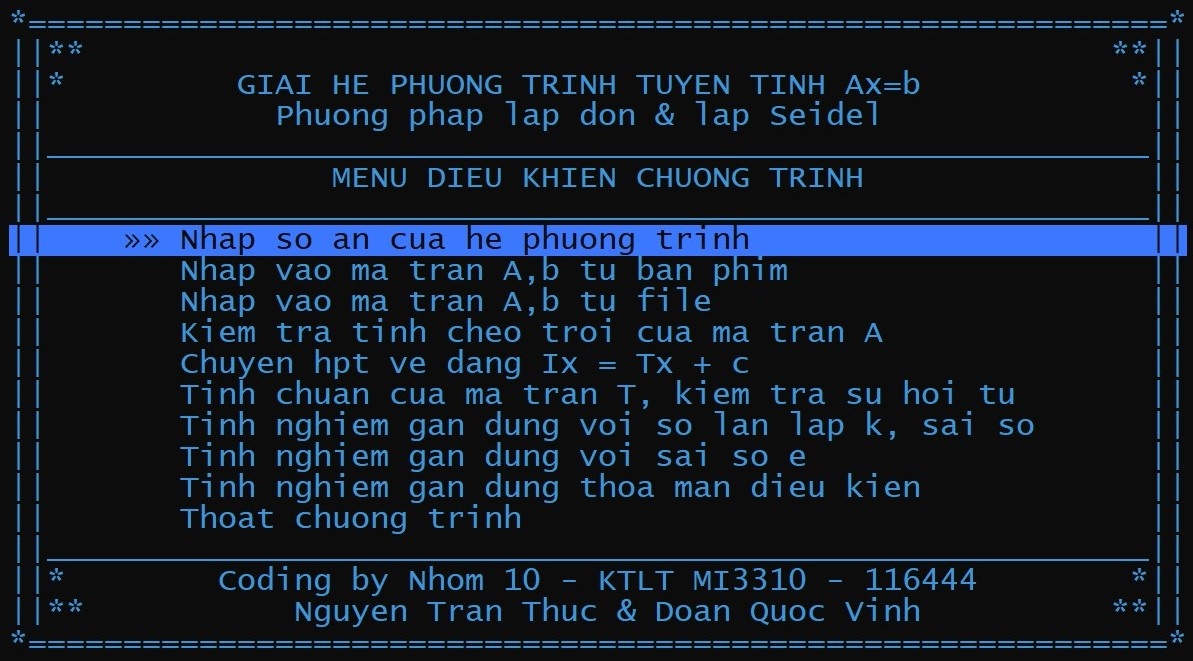
\includegraphics[scale=0.4]{figures/fig1}
\caption{Menu điều khiển chương trình}
\end{figure}


\begin{figure}[!h]
\label{fig:33}
\centering
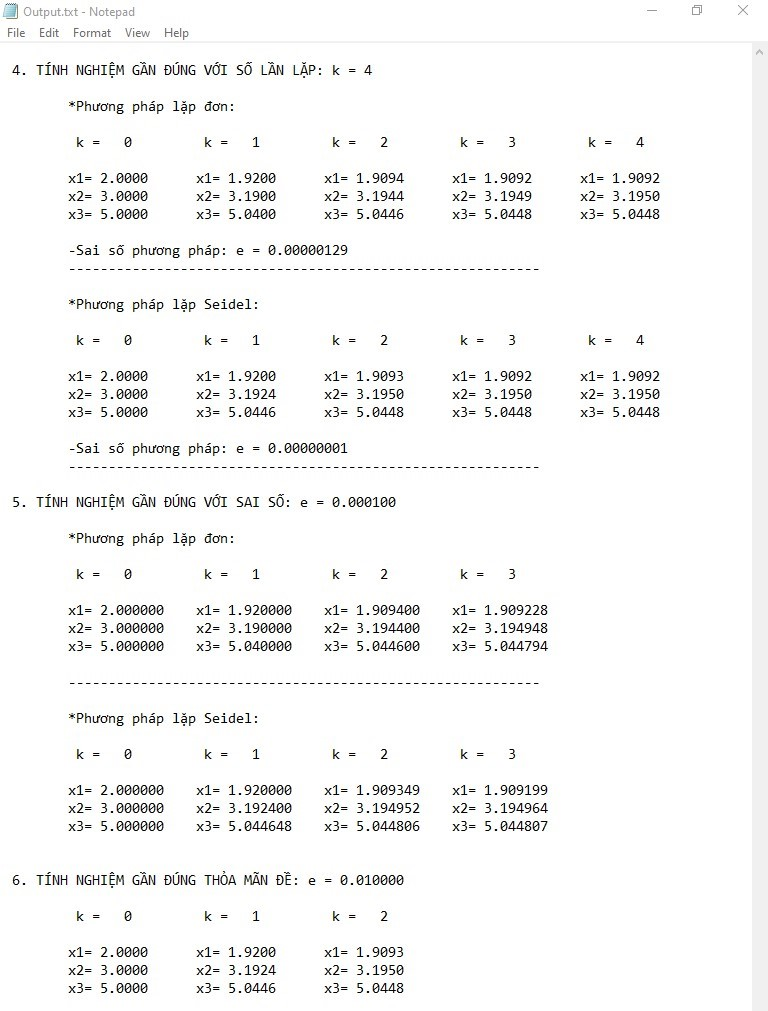
\includegraphics[scale=0.6]{figures/fig2}
\caption{Kết quả in ra tệp văn bản}
\end{figure}






\end{document}